\documentclass[]{article}
\newcommand{\FileDepth}{../..}
\usepackage[a4paper, total={15cm,23cm}]{geometry}
\usepackage[T1]{fontenc}
\usepackage{textcomp}%Not strictly necessary, but gives \textmu command for "micro."
\usepackage{fancyhdr}
\usepackage{amsmath}
\usepackage{amssymb}
\usepackage{graphicx}
\usepackage{xcolor}
\usepackage{tikz}
\usetikzlibrary{calc}
%opening
\newcommand{\SecType}{X}
\newcommand{\Week}{X}
\title{Representations of Vectors}
\author{Benjamin Bauml}
\date{Summer 2024}
\pagestyle{fancy}
\rhead{PH 211}
\chead{Summer 2024}
\lhead{Week \Week}

% For Assignment, leave Purpose as 1. For Worksheet, set to 2. For Student Solution, set to 3. For Teacher Solution, set to 4.
% If you want keep the pieces from being called manually, set DefOnly to 0.
\newcommand{\Purpose}{4}
\newcommand{\DefOnly}{1}

% Version 2024-04-27
% Changes
% 2024-02-21 Added xstring package to enable smooth implementation of new \ModePage command.
% 2024-04-27 Set up to split activities and formatting aspects into separate files. Removed dependence on xcomment. Added an automatic counter to number the activities in a problem set.
% 2024-05-19 Revised old format for \TeachingTips command, which did not support \DefOnly.
\usepackage{tcolorbox}
\usepackage{xstring}
% You will want the following four lines in your document (the last two uncommented):
% For Assignment, leave Purpose as 1. For Worksheet, set to 2. For Student Solution, set to 3. For Teacher Solution, set to 4.
% If you want keep the pieces from being called manually, set DefOnly to 0.
%\newcommand{\Purpose}{4}
%\newcommand{\DefOnly}{1}
\newcommand{\Exclusion}{0}
\newcommand{\PageTurn}{0}
\newcommand{\GrayProb}{0}
\newcommand{\Tipsy}{0}

% Assignment
\if\Purpose1
\renewcommand{\Exclusion}{1}
\fi
% Worksheet
\if\Purpose2
\renewcommand{\Exclusion}{1}
\renewcommand{\PageTurn}{1}
\fi
% Student Solution
\if\Purpose3
\renewcommand{\PageTurn}{1}
\renewcommand{\GrayProb}{1}
\fi
% Teaching Copy
\if\Purpose4
\renewcommand{\PageTurn}{1}
\renewcommand{\GrayProb}{1}
\renewcommand{\Tipsy}{1}
\fi

\def \NewQ {0}
\def \PForce {0}
\newcommand{\MaybePage}[1]{
	\def \PForce {#1}
	\if\PForce1
	\newpage
	\else
	\if\NewQ0
	\gdef \NewQ {\PageTurn}
	\else
	\newpage
	\fi
	\fi
}

\newcommand{\ModePage}[1]{
	\IfSubStr{#1}{\Purpose}{\newpage}{}
}

\newcounter{ActNumber}
\setcounter{ActNumber}{0}

\newcommand{\Problem}[4][0]{%The first argument is optional, and if it is set to 1, the \newpage will be forced. The second argument is the name of the activity, the third is the command the activity is stored as, and the fourth is the actual problem statement.
\newcommand{#3}{
\MaybePage{#1}
\addtocounter{ActNumber}{1}
\section*{\SecType\Week-\theActNumber: #2}
\if\GrayProb1
\begin{tcolorbox}[colback=lightgray,colframe=lightgray,sharp corners,boxsep=1pt,left=0pt,right=0pt,top=0pt,bottom=0pt,after skip=2pt]
\else
\begin{tcolorbox}[colback=white,colframe=white,sharp corners,boxsep=1pt,left=0pt,right=0pt,top=0pt,bottom=0pt,after skip=2pt]
\fi
#4
\end{tcolorbox}\noindent
}
\if\DefOnly0
\else
#3
\fi
}
	
\newcommand{\ProblemSub}[3][0]{%The first argument is optional, and if a string of numbers is entered into it, it will force a \newpage in any \Purpose that shows up in the string. For example, "13" would lead to the newpage being forced in modes 1 and 3. The second is the command the activity is stored as, and the third is the actual problem statement.
\newcommand{#2}{
\ModePage{#1}
\if\GrayProb1
\begin{tcolorbox}[colback=lightgray,colframe=lightgray,sharp corners,boxsep=1pt,left=0pt,right=0pt,top=0pt,bottom=0pt,after skip=2pt]
\else
\begin{tcolorbox}[colback=white,colframe=white,sharp corners,boxsep=1pt,left=0pt,right=0pt,top=0pt,bottom=0pt,after skip=2pt]
\fi
#3
\end{tcolorbox}\noindent
}
\if\DefOnly0
\else
#2
\fi
}
		
\newcommand{\Solution}[2]{%The first argument is the command the solution is stored as, and the second is the actual solution.
\newcommand{#1}{
\if\Exclusion0
#2
\fi
}
\if\DefOnly0
\else
#1
\fi
}
		
\newcommand{\ProblemFig}[2]{%The first argument is the command the figure is stored as, and the second is the actual figure.
\newcommand{#1}{
\begin{figure}[h]
#2
\end{figure}
}
\if\DefOnly0
\else
#1
\fi
}

\newcommand{\TeachingTips}[2]{%The first argument is the command the tip is stored as, and the second is the actual tip.
\newcommand{#1}{
\if\Tipsy1
\begin{tcolorbox}[colback=lightgray,colframe=black]
#2
\end{tcolorbox}
\fi
}
\if\DefOnly0
\else
#1
\fi
}

%\newcommand{\FBDaxes}[3]{
	\begin{scope}[shift={(#1)},rotate=#2]
		% x-axis
		\draw[thick,->] (-2,0) -- (2,0);
		\node[anchor=west] at (2,0) {$x$};
		% y-axis
		\draw[thick,->] (0,-2) -- (0,2);
		\node[anchor=west] at (0,2) {$y$};
		\coordinate (#3) at (0,0);
	\end{scope}
}
\newcommand{\FBDvectorMA}[4]{
	\begin{scope}[shift={(#1)}]
		\coordinate (#4tip) at ({#2*cos(#3)},{#2*sin(#3)});
		\draw[ultra thick,blue,->] (#1) -- (#4tip);
	\end{scope}
}
\newcommand{\FBDvectorXY}[3]{
	\begin{scope}[shift={(#1)}]
		\coordinate (#3tip) at (#2);
		\draw[ultra thick,blue,->] (0,0) -- (#3tip);
	\end{scope}
}
\newcommand{\FBDdot}[1]{
	\filldraw[black] (#1) circle (3pt);
}
%\newcommand{\MVec}[3][0]{%Creates a momentum vector of length #3 centered at #2 and rotated #1 degrees counterclockwise.
	\begin{scope}[rotate=#1,shift={(#2)}]
		\draw[->,thick] ({-#3/2},0) -- ({#3/2},0);
	\end{scope}
}
\newcommand{\MDot}[1]{%Creates a dot at #1 to represent a zero vector.
	\filldraw (#1) circle (1pt);
}
\newcommand{\MVDRows}[2][4.5]{%Creates the rows (initial, delta, final) of a momentum vector diagram. The optional argument determines the width of the table, and defaults to a good length for three columns (two objects and the total system). The non-optional argument gives a coordinate name (not displayed) to the diagram.
	\begin{scope}
		%\draw[thick] (0,5.5) -- (0,0);
		\draw[thick] (-1,4.5) -- (#1,4.5);
		\node at (-0.5,3.75) {$\vec{p}_{i}$};
		\draw[thick] (-1,3) -- (#1,3);
		\node at (-0.5,2.25) {$\Delta\vec{p}$};
		\draw[thick] (-1,1.5) -- (#1,1.5);
		\node at (-0.5,0.75) {$\vec{p}_{f}$};
		\coordinate (#2) at (0,5);
	\end{scope}
}
\newcommand{\MVDCol}[4][0.75]{%Creates a column for an object in a momentum vector diagram. The first (non-optional) argument is the coordinate name (not displayed) of the column, while the second is the displayed column header. The first argument also names the three entries down the column. The third argument anchors the column, so it should either be the coordinate name of the MVD (for the first column) or the coordinate name of the previous column. The optional argument indicates how far the center of the column should be from the previous column's edge, and defaults to 0.75
	\begin{scope}[shift={(#4)}]
		\node at (#1,0) {#3};
		%\draw[thick] ({#1*2},0.5) -- ({#1*2},-5);
		\draw[thick] (0,0.5) -- (0,-5);
		\coordinate (#2init) at (#1,-1.25);
		\coordinate (#2delt) at (#1,-2.75);
		\coordinate (#2fin) at (#1,-4.25);
		\coordinate (#2) at ({#1*2},0);
	\end{scope}
}

\begin{document}
\maketitle

\Problem{Represetations of Vectors}{\VecRepsI}{
Discuss \textbf{vectors} with your group.
}
\ProblemSub{\VecRepsII}{
Write down a list of things about vectors on your shared whiteboard. You can write:
\begin{itemize}
	\item words or sentences
	\item numbers or symbols
	\item pictures or diagrams
\end{itemize}
Write large!
}
\Solution{\VecRepsSol}{

The following list only contains my thoughts about vectors. It should not be assumed to be definitive. There are many other things about vectors that could have been included.
\begin{itemize}
	\item A vector has direction and magnitude.
	\item A vector is often represented with an arrow; the length is its magnitude, and the orientation of the arrow (its angle) indicates direction.
	\begin{center}
		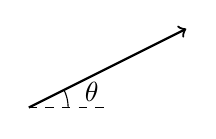
\begin{tikzpicture}
			\draw[thick,->] (0,0) -- (2,1);
			\draw[dashed] (0,0) -- (1,0);
			\draw (0.5,0) arc (0:27:0.5);
			\node at (0.8,0.2) {$\theta$};
		\end{tikzpicture}
	\end{center}
	\item Vectors add ``tip-to-tail.''
	\begin{center}
		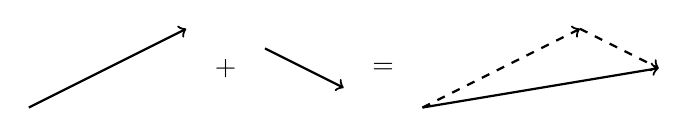
\begin{tikzpicture}
			\draw[thick,->] (0,0) -- (2,1);
			\node at (2.5,0.5) {$+$};
			\draw[thick,->,shift={(3,0)}] (0,0.75) -- (1,0.25);
			\node at (4.5,0.5) {$=$};
			\draw[thick,->,shift={(5,0)}] (0,0) -- (3,0.5);
			\draw[thick,dashed,->,shift={(5,0)}] (0,0) -- (2,1);
			\draw[thick,dashed,->,shift={(7,0.25)}] (0,0.75) -- (1,0.25);
		\end{tikzpicture}
	\end{center}
	\item Multiplying a vector by a scalar changes its length.
	\begin{center}
		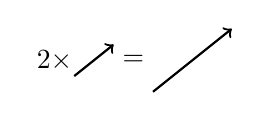
\begin{tikzpicture}
			\node at (0,0) {$2\times$};
			\draw[thick,->] (0.25,-0.2) -- (0.75,0.2);
			\node at (1,0) {$=$};
			\draw[thick,->] (1.25,-0.4) -- (2.25,0.4);
		\end{tikzpicture}
	\end{center}
	\item Multiplying a vector by $-1$ reverses its direction.
	\begin{center}
		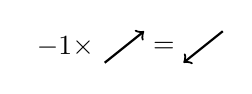
\begin{tikzpicture}
			\node at (-0.25,0) {$-1\times$};
			\draw[thick,->] (0.25,-0.2) -- (0.75,0.2);
			\node at (1,0) {$=$};
			\draw[thick,->] (1.75,0.2) -- (1.25,-0.2);
		\end{tikzpicture}
	\end{center}
	\item Vectors can be broken into components.
	\begin{center}
		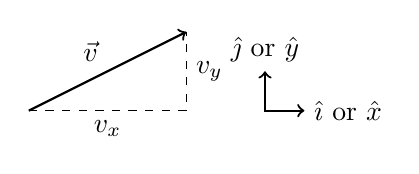
\begin{tikzpicture}
			\draw[thick,->] (0,0) -- (2,1);
			\node[anchor=south east] at (1,0.5) {$\vec{v}$};
			\draw[dashed] (0,0) -- (2,0) -- (2,1);
			\node[anchor=north] at (1,0) {$v_{x}$};
			\node[anchor=west] at (2,0.5) {$v_{y}$};
			\draw[<->,thick] (3,0.5) -- (3,0) -- (3.5,0);
			\node[anchor=south] at (3,0.5) {$\hat{\jmath}$ or $\hat{y}$};
			\node[anchor=west] at (3.5,0) {$\hat{\imath}$ or $\hat{x}$};
		\end{tikzpicture}
	\end{center}
	Parenthetical or angle-bracket notation was probably used in your math classes:
	\[
	\vec{v} = (v_{x},v_{y}) = \langle v_{x},v_{y}\rangle.
	\]
	It is okay, but parentheses and angle brackets can mean a lot of things, so it may not always be clear. \\
	We recommend unit vector notation, as it is much clearer:
	\[
	\vec{v} = v_{x}\hat{\imath} + v_{y}\hat{\jmath} = v_{x}\hat{x} + v_{y}\hat{y}.
	\]
	Using $\hat{x}$, $\hat{y}$, $\hat{z}$ instead of $\hat{\imath}$, $\hat{\jmath}$, $\hat{k}$ helps to more clearly associate the Cartesian unit vectors with the coordinate axes. \\
	\textbf{Warning!} Cosine is not always $x$! It depends on where the angle is.
	\begin{center}
		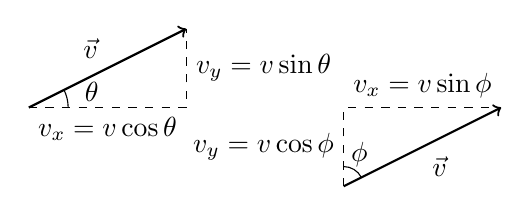
\begin{tikzpicture}
			\begin{scope}[shift={(-2,0.5)}]
				\draw[thick,->] (0,0) -- (2,1);
				\node[anchor=south east] at (1,0.5) {$\vec{v}$};
				\draw[dashed] (0,0) -- (2,0) -- (2,1);
				\draw (0.5,0) arc (0:27:0.5);
				\node at (0.8,0.2) {$\theta$};
				\node[anchor=north] at (1,0) {$v_{x}=v\cos\theta$};
				\node[anchor=west] at (2,0.5) {$v_{y}=v\sin\theta$};
			\end{scope}
			\begin{scope}[shift={(2,-0.5)}]
				\draw[thick,->] (0,0) -- (2,1);
				\node[anchor=north west] at (1,0.5) {$\vec{v}$};
				\draw[dashed] (0,0) -- (0,1) -- (2,1);
				\draw (0,0.25) arc (90:27:0.25);
				\node at (0.2,0.4) {$\phi$};
				\node[anchor=south] at (1,1) {$v_{x}=v\sin\phi$};
				\node[anchor=east] at (0,0.5) {$v_{y}=v\cos\phi$};
			\end{scope}
		\end{tikzpicture}
	\end{center}
	\item Vectors add ``componentwise.''
	\begin{center}
		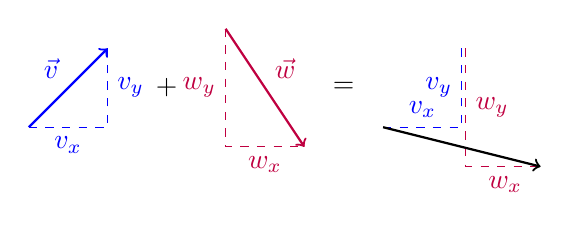
\begin{tikzpicture}
			\begin{scope}[blue,shift={(0,0)}]
				\draw[thick,->] (0,0) -- (1,1);
				\node[anchor=south east] at (0.5,0.5) {$\vec{v}$};
				\draw[dashed] (0,0) -- (1,0) -- (1,1);
				\node[anchor=north] at (0.5,0) {$v_{x}$};
				\node[anchor=west] at (1,0.5) {$v_{y}$};
			\end{scope}
			\node at (1.75,0.5) {$+$};
			\begin{scope}[purple,shift={(2.5,0.25)}]
				\draw[thick,->] (0,1) -- (1,-0.5);
				\node[anchor=south west] at (0.5,0.25) {$\vec{w}$};
				\draw[dashed] (0,1) -- (0,-0.5) -- (1,-0.5);
				\node[anchor=north] at (0.5,-0.5) {$w_{x}$};
				\node[anchor=east] at (0,0.25) {$w_{y}$};
			\end{scope}
			\node at (4,0.5) {$=$};
			\begin{scope}[blue,shift={(4.5,0)}]
				%\draw[thick,->] (0,0) -- (1,1);
				%\node[anchor=south east] at (0.5,0.5) {$\vec{v}$};
				\draw[dashed] (0,0) -- (1,0) -- (1,1);
				\node[anchor=south] at (0.5,0) {$v_{x}$};
				\node[anchor=east] at (1,0.5) {$v_{y}$};
			\end{scope}
			\begin{scope}[purple,shift={(5.55,0)}]
				%\draw[thick,->] (0,1) -- (1,-0.5);
				%\node[anchor=south west] at (0.5,0.25) {$\vec{w}$};
				\draw[dashed] (0,1) -- (0,-0.5) -- (0.95,-0.5);
				\node[anchor=north] at (0.5,-0.5) {$w_{x}$};
				\node[anchor=west] at (0,0.25) {$w_{y}$};
			\end{scope}
			\draw[thick,->] (4.5,0) -- (6.5,-0.5);
		\end{tikzpicture}
	\end{center}
	\[
	{\color{blue}\vec{v}} + {\color{purple}\vec{w}} = {\color{blue}v_{x}\hat{x}+v_{y}\hat{y}} + {\color{purple}w_{x}\hat{x}+w_{y}\hat{y}} = ({\color{blue}v_{x}}+{\color{purple}w_{x}})\hat{x} + ({\color{blue}v_{y}}+{\color{purple}w_{y}})\hat{y}
	\]
\end{itemize}
}
\end{document}